% Author: Thomas Barratt
% Version: 1.0
% This work is licensed under a Creative Commons Attribution 4.0 International License.

\documentclass[11pt, a4paper, titlepage]{article}
% \usepackage[T1]{fontenc}
% \usepackage[latin1]{inputenc}
\usepackage[english]{babel}
\usepackage{siunitx}
\usepackage{graphicx}
\usepackage{tipa} % for the \ark{} command
\usepackage{graphics} % for pdf, bitmapped graphics files
% \usepackage{times} % assumes new font selection scheme installed
\usepackage{amsmath}
\usepackage{latexsym}
\usepackage{amscd}% for commutative diagrams
% \usepackage{mathrsfs} %this package is for the script font \mathscr
\usepackage{relsize}
\usepackage{delarray}
\usepackage{pstricks}
\usepackage{theorem}
\usepackage{changepage}
\usepackage{euscript}
% \usepackage{textcomp}
\usepackage{esvect}
\usepackage{parskip}
\usepackage{placeins}
\usepackage{subfigure}
% \usepackage{subcaption}
\usepackage{array}
\usepackage{delarray}
\usepackage{stmaryrd}
\usepackage{fancyhdr}
\usepackage{graphpap}
\usepackage{makeidx}
\usepackage{enumerate}
\usepackage{esint}
\usepackage{datetime}
\usepackage{caption}
\usepackage{smartdiagram}
\usesmartdiagramlibrary{additions}
%Set Abstract Page
\usepackage{abstract}
\setlength{\absleftindent}{-5mm}
\setlength{\absrightindent}{-5mm}

%Colour definitions - put before TikZ
\usepackage{color}
\definecolor{igreen}{rgb}{0.0, 0.56, 0.0}
\usepackage{xcolor, colortbl}
\colorlet{gred}{-red!75!green!65!}
\colorlet{mamber}{-red!75!green!15!blue!50!}
\colorlet{grown}{-red!75!blue!20!green}
\colorlet{bled}{-red!85!blue!40!green!45!}
\colorlet{waters}{cyan!25} % Define color for the water
\colorlet{water}{cyan!25!green!20!} % Define color for the water
\definecolor{grin}{HTML}{00F9DE}
\usepackage{rotating}
\providecommand{\keywords}[1]{\textbf{\textit{Keywords---}} #1}

% For faint dotted table line
\usepackage{arydshln}
\setlength{\dashlinedash}{.4pt}
\setlength{\dashlinegap}{.8pt}

\usepackage{booktabs}
\usepackage{graphicx}
\usepackage{tikz}
\usepackage{tikz-3dplot}
\usetikzlibrary{
arrows,
arrows.meta,
automata,
backgrounds,
calc,
decorations,
decorations.pathmorphing,
decorations.pathreplacing,
decorations.fractals,
external,
fit,
matrix,
petri,
positioning,
shadows,
shapes,
shapes.multipart,
topaths,
intersections
}
\usepackage{eso-pic}
\def\ba{\begin{array}}
\def\ea{\end{array}}
\def\beann{\begin{eqnarray*}}
\def\eeann{\end{eqnarray*}}
\def\bea{\begin{eqnarray}}
\def\eea{\end{eqnarray}}
\def\bsy{\boldsymbol}
\def\gray#1{{\color{gray}#1}}

%% COUNTERS
\setcounter{MaxMatrixCols}{20}
% \renewcommand{\thesection}{\arabic{section}}
% \renewcommand{\thesection}{\thechapter.\number\numexpr\value{section}}
% \renewcommand{\thesubsection}{\thesection.\number\numexpr\value{subsection}}
%%For changemargin
% \def\quote{\list{}{\rightmargin\leftmargin}\item[]}
% \let\endquote=\endlist 
% \def\changemargin#1#2{\list{}{\rightmargin#2\leftmargin#1}\item[]}
% \let\endchangemargin=\endlist 
% \makeatletter
% \newlength\qvec@height
% \newlength\qvec@depth
% \newlength\qvec@width
% \newcommand{\qvec}[2][]{
%     \settoheight{\qvec@height}{$#2$}
%     \settodepth{\qvec@depth}{$#2$}
%     \settowidth{\qvec@width}{$#2$}
%   \def\qvec@arg{#1}
%   \raisebox{.2ex}{\raisebox{\qvec@height}{\rlap{% 
%     \kern.05em
%     \begin{tikzpicture}[scale=1,shorten >=-3pt,shorten <=-3pt]
%     \pgfsetroundcap
%     \coordinate (Stx) at (.05em,0) ;
% 		\coordinate (Arx) at (\qvec@width-.05em,0) ;
%     \draw[->](Stx) to[bend left] (Arx);
%     \end{tikzpicture}
%   }}}
%   #2
% }
% \makeatother
% \makeatletter
% \newlength\pvec@height
% \newlength\pvec@depth
% \newlength\pvec@width
% \newcommand{\pvec}[2][]{
%     \settoheight{\pvec@height}{$#2$}
%     \settodepth{\pvec@depth}{$#2$}
%     \settowidth{\pvec@width}{$#2$}
%   \def\pvec@arg{#1}
%   \raisebox{.2ex}{\raisebox{\pvec@height}{\rlap{% 
%     \kern.05em
%     \begin{tikzpicture}[scale=1,shorten >=-3pt,shorten <=-3pt]
%     \pgfsetroundcap
%     \coordinate (Stx) at (.05em,0) ;
% 		\coordinate (Arx) at (\pvec@width-.05em,0) ;
%     \draw[->](Stx) to[bend right] (Arx);
%     \end{tikzpicture}
%   }}}
%   #2
% }
% \makeatother
% \makeatletter
% \newlength\vvec@height%
% \newlength\vvec@depth%
% \newlength\vvec@width%
% \newcommand{\vvec}[2][]{%
%   \ifmmode%
%     \settoheight{\vvec@height}{$#2$}%
%     \settodepth{\vvec@depth}{$#2$}%
%     \settowidth{\vvec@width}{$#2$}%
%   \else 
%     \settoheight{\vvec@height}{#2}%
%     \settodepth{\vvec@depth}{#2}%
%     \settowidth{\vvec@width}{#2}%
%   \fi%
%   \def\vvec@arg{#1}%
%   \def\vvec@dd{:}%
%   \def\vvec@d{.}%
%   \raisebox{.2ex}{\raisebox{\vvec@height}{\rlap{%
%     \kern.05em%
%     \begin{tikzpicture}[scale=1]
%     \pgfsetroundcap
%     \draw (.05em,0)--(\vvec@width-.05em,0);
%     \draw (\vvec@width-.05em,0)--(\vvec@width-.15em, .075em);
%     \draw (\vvec@width-.05em,0)--(\vvec@width-.15em,-.075em);
%     \ifx\vvec@arg\vvec@d%
%       \fill(\vvec@width*.45,.5ex) circle (.5pt);%
%     \else\ifx\vvec@arg\vvec@dd%
%       \fill(\vvec@width*.30,.5ex) circle (.5pt);%
%       \fill(\vvec@width*.65,.5ex) circle (.5pt);%
%     \fi\fi%
%     \end{tikzpicture}%
%   }}}%
%   #2%
% }
\makeatother
\def\ba{\begin{array}}
\def\ea{\end{array}}
\def\beann{\begin{eqnarray*}}
\def\eeann{\end{eqnarray*}}
\def\bea{\begin{eqnarray}}
\def\eea{\end{eqnarray}}
\def\bsy{\boldsymbol}
\def\gray#1{{\color{gray}#1}}
% \usepackage{titlesec}
\usepackage{multirow}
%To reference within text
\usepackage{hyperref}
\usepackage{apacite}
\usepackage{lipsum}
\usepackage{tikz-cd}
\usepackage{float}
% \usepackage{titling}
\usepackage{epigraph}
\usepackage[title, titletoc]{appendix}
\setlength\epigraphwidth{8cm}
\setlength\epigraphrule{0pt}

% \titleformat{\chapter}{\normalfont\LARGE}{\thechapter\,$\vert$}{20pt}{\LARGE}{\setcounter{chapter}{0}}
\setlength{\headheight}{15pt}
% \titlespacing*{\chapter}{0pt}{-70pt}{40pt} %Move chapter titles up
% Title page logos:
% \makeatletter
% \newcommand\BackgroundPicturea[3]{
% 	\setlength{\unitlength}{1pt}
% 	\put(0,\strip@pt\paperheight){
% 		\parbox[t]{\paperwidth}{
% 			\vspace{#2}\hspace{#3}
% 			\mbox{\includegraphics[scale=0.5]{#1}}
% }}}
% \newcommand\BackgroundPictureb[3]{
% 	\setlength{\unitlength}{1pt}
% 	\put(0,\strip@pt\paperheight){
% 		\parbox[t]{\paperwidth}{
% 			\vspace{#2}\hspace{#3}
% 			\mbox{\includegraphics[scale=0.3]{#1}}
% }}}
\makeatother
% For my abbreviations
\newcommand{\abbrlabel}[1]{\makebox[3cm][l]{\textbf{#1}\ \dotfill}}
\newenvironment{abbreviations}{\begin{list}{}{\renewcommand{\makelabel}{\abbrlabel}}}{\end{list}}
% Line Spacing
\usepackage{setspace}
\setstretch{1.1}
%Set of command is for the changemargin environment
\def\quote{\list{}{\rightmargin\leftmargin}\item[]}
\let\endquote=\endlist 
\def\changemargin#1#2{\list{}{\rightmargin#2\leftmargin#1}\item[]}
\let\endchangemargin=\endlist
%Replace Contents to Table of Contents	
\addto\captionsenglish{
	\renewcommand{\contentsname}%
	{Table of Contents}
	\setcounter{tocdepth}{3}% Include \subsubsection in ToC
	\setcounter{secnumdepth}{3}% Number \subsubsection in ToC
	}
\renewcommand{\listfigurename}{List of Figures}
\renewcommand{\listtablename}{List of Tables}
\usepackage{geometry}
\usepackage{csquotes}
\usepackage{mathtools}
\usepackage{multicol}
\usepackage{hyperref}
\usepackage{apacite}
\usepackage[title, titletoc]{appendix}
\usepackage[parfill]{parskip}
\usepackage{array,etoolbox}
\usepackage{float}
\preto\tabular{\setcounter{magicrownumbers}{0}}
\newcounter{magicrownumbers}
\newcommand\rownumber{\stepcounter{magicrownumbers}\arabic{magicrownumbers}}

\DeclareUnicodeCharacter{00A0}{ }
\geometry{lmargin=1in, rmargin=1in} 

% Better inline directory listings
\usepackage{xcolor}
\definecolor{light-gray}{gray}{0.95}
\newcommand{\code}[1]{\colorbox{light-gray}{\texttt{#1}}}
 
% \hypersetup{pdftitle = Applications of Cellular Automata: Wildfire Spread simulation, pdfauthor = {Thomas Barratt, Jacob Dalrymple}, pdfstartview=FitH, pdfkeywords = essay, pdfpagemode=FullScreen, colorlinks, anchorcolor = red, citecolor = blue, urlcolor=blue, filecolor=green, linkcolor=red, plainpages=false}
%%%%%%%%%%%%%%%%%%%%%%%%%%%%%%%%%%%%%%%%%%%%%%%%%%%%%%%%%%%%%%%%%%%%%%%
% \pagestyle{fancy}

% Top and Bottom Line Rules
% \renewcommand{\headrulewidth}{0.4pt} %0.4pt
% \renewcommand{\footrulewidth}{0.4pt}
% \fancyheadoffset{9pt}
% \fancyfootoffset{9pt}
% Line spacing
\renewcommand{\baselinestretch}{1.1} %1.5
%%%%%%%%%%%%%%%%%%%%%%%%%%%%%%%%%%%%%%%%%%%%%%%%%%%%%%%%%%%%%%%%%%%%%%%
\date{}

\title{ \textbf{Applications of Cellular Automata: Wildfire Spread simulation} \\  }

\author{\\ \Large{Thomas Barratt, Jacob Dalrymple  } }
\date{\today}
%%%%%%%%%%%%%%%%%%%%%%%%%%%%%%%%%%%%%%%%%%%%%%%%%%%%%%%%%%%%%%%%%%%%%%%
% \pagenumbering{roman}
\begin{document}
\maketitle

\newpage

\section{Abstract}
This project seeks to expand an existing Cellular Automata Game of Life system developed in \cite{capyle_home_2016} to investigate the effects of differing environmental parameters on a forest fire across a fixed terrain.

By constructing a probabilistic model which takes into account parameters pertinent to fire spread (wind speeds and terrain heights, flammability of different plant life), results which concur with the current body of research have been generated.

\section{Introduction}
By implementing a 6-state based model of fire spread across a variable-height terrain with wind and areas of varying flammability, we have been able to simulate the spread of a real forest fire across a simulated environment, dictated by the specification given.

By using a minimal state set and an ancillary 20-value cell attribute grid, we can model complex relationships between the properties of an area in a forest fire to create a stochastic state transition function for each cell in the next time step.

Attempting to relate our simulation to the real world values of forest fires across a similar terrain, we have gradually improved the weighting of various factors to generate a suitable fire spread. 
% \newpage
\section{Background: Literature Review}
% \begin{displayquote}
%   Your brief restatement of the problem
%   that you have been asked to solve. Carry out a search of the literature to identify at least two
%   examples of journal papers that describe CA-based models relevant to this system. What features
%   did they model? What did they predict?
% \end{displayquote}
Consulting existing research into the field of cellular automata can give us a valuable insight into how best to proceed when considering the formulation of a model which can describe the spread of wildfire. Considering what properties are being modelled and the ways in which transitions between state are decided can give us a grounding in this specific problem area. Research into the real world applications of forest fires are fruitful and well explored: using CA to explore forest fires is something that is well researched [\cite{ntinas2017parallel}
\cite{clarke1994cellular}
\cite{trunfio2011new}].

Considering the evidence existing papers have used to justify their results, including their empirical values formulated by authors familiar with the problem domain, can provide a good metric for the accuracy of our results. 

% Because this project seeks to show the effect of wildfires in relation to a municipality and surrounding area,the real world implications are obvious, and should be considered throughout our research into this domain.

There are two notable papers in this field whose outcomes seem to overlap strongly with our intentions. Both of these papers consider simulating real world forest fires using cellular automata, but have different approaches to the use of neighbourhoods and states, and their relationship with the real world properties that affect forest fires.


\cite{HERNANDEZENCINAS20071213} seeks to model forest fires using a hexagonal grid, modeling various different fuel values as states. By using a hexagonal model, the size of each cells' neighbourhood is increased - allowing more complex calculations to be derived on the basis of a `near neighbourhood' and `distant neighbourhood'.
The authors of the paper opt to use 3 properties when considering the flammability rate of a cell: wind, topography, and the rate of fire speed. This simplistic model differs from that of \cite{ALEXANDRIDIS2008191}, which includes 
spread and shape of a forest fire front; the fuel type (type of vegetation); humidity; wind direction and magnitude; terrain topography (slope and natural barriers), fuel continuity (vegetation thickness); and spotting - a phenomenon where burning material is transferred by the wind or other reasons such as the fling of flaming pinecones to areas that are not adjacent to the fire front.

Although the inclusion of additional parameters in \cite{ALEXANDRIDIS2008191} allows an implementation with greater accuracy in relation to real forest fires, this is only true if the correct relationships and weightings are defined.

    % \begin{itemize}
    %   \item Wind
    %   \item Topography
    %   \item Rate of fire spread
    % \end{itemize}

  \cite{HERNANDEZENCINAS20071213} following states are defined in the paper: \\ $\left\{ 0, 0.1, 0.2, 0.3, 0.4, 0.5, 0.6, 0.7, 0.8, 0.9, 1  \right\}$, where each value represents a fuel value. This differs from \cite{ALEXANDRIDIS2008191}, where four states were used ($ \left\{ 0, 1, 2,3 \right\}$), which represent differing functional states. This choice of state representation is based on the paper's approach to the functional implementation of what means to `be on fire'.

 \cite{ALEXANDRIDIS2008191}'s model was designed to include the most impactful properties when considering the spread of wildfire. By comparing their results against that of the 1990 Spetses island wildfires, and iteratively changing constants in their transition functions, the authors simulated forest fire spread to a high degree of accuracy - their final results occupying $5.4km^2$, with the actual fire occupying $5.9km^2$.

 To calculate the chance of a cell being `on fire', \cite{HERNANDEZENCINAS20071213} uses the following approach. Each parameter [listed above] is given a weighting and a probablistic model is used for each parameter to calculate the total chance of a cell being set on fire in the next time step ($t+1$).

 The chance of fire, $p_{burn}$, is given as:

 \[ p_{burn} = p_h(1+p_{veg})(1+p_{den})p_wp_s \]
 where: \\
 $p_h = $ constant probability that a cell adjacent to a burning cell containing a given type of vegetation and density will catch fire at the next time step under no wind and flat terrain \\
 $p_{den}, p_{veg}, p_w, p_s$ = the density of vegetation, the type of vegetation, the wind speed and the slope, respectively.

 In contrast, \cite{HERNANDEZENCINAS20071213} looked to find the optimal values in any forest fire, using purely mathematical models which consider heavily the boundary conditions of each of the hexagon cells in an inhomogeneous forest neighborhood.

 This difference in approach, applied versus maximum mathematical, shows the effect of the fuzzy nature of real life. \cite{ALEXANDRIDIS2008191}, which looked towards a case study to generate its values, relied on empirical constants, whereas \cite{HERNANDEZENCINAS20071213} focused entirely on a formulaic approach.

 When considering the use of CA in our study, the question of whether a case study based approach has to be answered. Due to the greater knowledge of the existing authors on the topic, ensuring the work presented here is the best position to build on their findings is essential.

  % \cite{ALEXANDRIDIS2008191}  defines the following relationship between the neighborhood of a cell and its state: If all cells in the neighborhood of $O = (a, b)$ are unburned at time $t$ except only one adjacent cell, which is completely burned out, then at time $t + 1$, the cell $(a, b)$ is completely burned out.
 

  
    % The authors states several key criteria which affect the spread of wildfire across a terrain.

  The use of additional parameters such as humidity to predict the spread of the forest fire, along with their use of real world GIS values gives rise to a greater accuracy of results (in relation to the real world spread of forest fires) when compared to the default criteria to be implemented.

  To meet the criteria given, the insights regarding the weighting of different parameters and the use of a probabilistic model to calculate the chance of a cell burning offer a credible starting point.

  The two papers discussed above implement the idea of 'fuel' in different ways. \cite{ALEXANDRIDIS2008191} structures fuel as a property of the states, whereas \cite{HERNANDEZENCINAS20071213} provides different states for different levels of fuel. 
  
  The advantage of moving the fuel state into an attribute of the cell is the greater precision of fuel that can be stored, while also maintaining a smaller amount of states. By limiting fuel state to discrete variables, the forest fire spread will lose valuable resolution which can be maintained with a different data structure.
% \newpage
\section{Methodology}
% \begin{displayquote}
%   - A short summary (IN YOUR OWN WORDS) of how the CA approach can
%   be applied to model a forest fire. This should assume that the reader is a non-expert in modelling or
%   Computer Science in general. You should explain in English (as opposed to simply using code), how
%   you have extended the model you have been given in order to investigate the features mentioned.
%   You can also use simple flow or state transition diagrams to support you description. You can also
%   refer to relevant python code included in an appendix.
%   It is expected that in extending/developing your model you will have to make some assumptions
%   about how to implement particular behaviours, and also in terms of the parameters (values) you
%   choose to use e.g. to represent different fuel resources/burning times. You are not expected to
%   become experts in this area but you should at state justify any assumptions you make.
% \end{displayquote} 

Cellular Automata is a term to describe the simulation of a discrete number of cells and interactions across a cell space (grid). Each cell can have one state at any one time step (generation). Cells can change state. The permitted changes from any one state to another state is determined by a transition function. The transition function can consider global properties, such as the current time step, as well as local properties, such as the cell's current state, as well as its neighbourhood - a set of cells near the cell. 

By representing small sections of the terrain as cells, cellular automata can be used to simulate the spread of the fire across the grid. The amount of cells can be thought of as the resolution of the simulation. 

After consulting existing literature, the following functional states were devised. 

\begin{enumerate}
  \setcounter{enumi}{-1}
  \item \textbf{Burnt out} - cells which were once on fire, but have no fuel remaining.
  \item \textbf{Burnable grass} - the default state for the terrain, as listed by the specification
  \item \textbf{Dense Forest} - Thick forest with more `fuel' than burnable grass, but which is harder to ignite.
  \item \textbf{High Flammable Scrub} - A low fuel but highly flammable substance, found in the valley in the specification
  \item \textbf{On fire} - cells which are on fire
  \item \textbf{Buildings} - cells which are buildings, this represents the town on the map.
  \item \textbf{Water} - a state which can never be on fire.
\end{enumerate}

These states represent the same approach as that of \cite{ALEXANDRIDIS2008191}, where each state represents a functionally different cell. This state model is an extension of a binary state CA given as a starting point for this assignment. The migration away from a two state model was necessary to capture the detail provided in the specification and also to implement some of the core findings from existing literature.

Burnable grass, Dense Forest and High Flammable Shrub are all variations of a burnable substance, and although this could be managed entirely within the attribute grid for each cell, having dedicated states allows the representation of the differing areas with different colours with the CaPyle simulation engine \cite{capyle_home_2016}. 

\begin{figure}[h]
  \centering
    \begin{tabular}{ || l | l ||}
      \hline
      \textbf{State}            &  \textbf{Valid transition states}  \\ 
      \hline
      Burnt Out        &  Burnt out           \\       
      Burnable grass         &  Burnable grass, On fire   \\
      On fire          &  On fire, Burnt out  \\   
      Buildings          &  Buildings, On fire  \\   
      Water     &  Water        \\
      \hline
 
    \end{tabular}
  \caption{Valid state transitions for each of the states in the CA.}
  \label{Valid state transitions}
\end{figure}

To produce a performant simulation which can cope with many generations, values which can be precomputed are done so in a setup function, and are then added to the attributes grid as an additional dimension.

The transitions between states are then calculated using these attributes for each cell (along with the local properties of the cell, such as number of neighbours in a certain state), which are stored in an $20$-value array for each cell in a grid equal in width and height to the grid. 

\begin{itemize}
  \item [0.] Height - Scalar value (m)
  \item [1.] Flammability
  \item [2.] Humidity
  \item [3.] Fuel
  \item [4-12.] Wind difference vectors (difference between wind in cell and neighbours) ($ms^{-1}$)
  \item [13-20.] Height difference vectors (difference between height in cell and neighbours) ($m$)
  % \item 8 Wind vectors 
  % \item 8 Height vectors  - assumption about heights
  % \item Flammability
  % \item Humidity
  % \item Fuel
\end{itemize}

In the current system, although humidity attributes are passed for every cell, they are not used when calculating the probability of ignition. This is an area that could be developed on with further investment. 

\subsection{Modelling the effect of wind in the model}
Wind has a significant effect on wildfires, with research suggesting that even a wind speed of $2$ to $6ms^{-1}$ can increase the spread of the fire by an additional 50\% \cite{Beer1991}. As wind heavily is discussed in both \cite{ALEXANDRIDIS2008191} and \cite{HERNANDEZENCINAS20071213}, factoring wind into this model would effectively build on their findings.

By computing 8 wind weights for each cell that affect the spread of fire in the 8 directions of the model, the directional influence the wind has on the fire front can be simulated. To calculate the wind's affect \cite{ALEXANDRIDIS2008191}'s method will be adapted for this implementation - by using the computed weights present within, we can measure the winds affect in meters per generation.

For every cell in the grid wind weights are calculated for each of the possible 8 directions the fire could be approaching .i.e North, East, North East etc.

By initially setting wind to be two scalars, an $\pm$ value for wind in the X axis, and in the Y axis, and then converting this to a vector, we can then find the angle between the wind vector $v_w$ and each of the fire direction vectors $v_f$ using the cosine rule:
\[\theta = \arccos{ \frac{v_w \cdot v_f}{|v_w||v_f|} }\]

The wind weight can be calculated using the formula:

\[w = \exp{(a_1 \cdot |v_w|)} \exp{(a_2 \cdot |v_w| \cdot (\cos(\theta) - 1))}\]

Where $a_1$ and $a_2$ are weights, calculated by \cite{ALEXANDRIDIS2008191}, which are derived from studying the growth of the 1992 Spetses Island forest fire.\\
These calculations can be done in the preprocessing steps before the simulation runs, reducing the computational complexity of the simulation.

\subsubsection{Modelling the effect of height in the model}
The implementation of height in this model begins with an assumption: rate of flammability is inversely proportional to the height difference.


In the setup phase, heights are defined for each cell. Each cell has access to the heights of its neighbours through the cell attributes grid. During the ignition probability calculation, the height weights can then be calculated from the values in the cell attributes grid (done so in the \code{cal\_height\_weight}). By calculating the difference in the heights between a cell and its neighborhood, a cell's chance of setting on fire can be affected by the number of on fire cells and this distance. 

\subsubsection{Modelling airdropped water}
As per the specification, ensuring we can air drop water at a custom time interval is required. To achieve this, allowing for a dynamic \code{time\_to\_drop} variable which can be adjusted has been added to the model.

By setting this to different intervals, we can see the effects of dropping water on the fire front.

\subsection{Calculating transitions}

Using the methods defined in \cite{ALEXANDRIDIS2008191} as a basis for our transitions, our grid is computed at every interval using two behaviours, \code{ignite} and \code{reduce\_fuel}, which perform as their names suggest, both returning new, computed versions of the grid.

\subsubsection{Ignite}
% Height

% Pass windx, windy, scalars, create vector from both  (Constant across all cells - vector), calculate magnitude of vector.
% Fire vectors calculated in neighbours N, NE, E....
% define angle array.
% Calculate difference in angle between the two.
% Supply wind vector and fire vector, calculate the angle difference, results in 8 different angle diffs, for each neighbour

% Uses formula to calculate the angular differences, and the wind vectors, using formula defined in \cite{ALEXANDRIDIS2008191}, we can plug in values:

% Weightings used in the paper.

% Result is wind weighting across all 8 different neighbours.

% Calculate wind weight, initially 0, (8,200,200), wind weight increased by number of neighbours on fire.

Ignite works by assigning a probability that a cell will transition into a burning state, the ignition probability of cell $c$ is calculated as follows:

\[ prob(c) = 0.5n(c)*f(c)*w(c)*h(c)*v \]

where $n(c)$ is returns a 1 if the cell has any on fire neighbours, or 0 if it has none; $f(c)$ is the rate of flammability for the cell (\code{rate\_of\_flam}); $w(c)$ is the wind weight for that cell; $h(c)$ is the height weight for the cell, and $v$ represents a degree of randomness.

The height weight for a cell is computed by comparing the current cell against its on fire neighbours' heights. For every neighbour that is on fire, the \code{height\_weight} is increased by a factor of the height difference ($0.0051 *$ height difference).  

Similarly, the wind weight for a cell is computed by consulting the 8-dimensional wind magnitude grid attributes generated at setup. For each on fire neighbour of a cell, the associated wind value from the 8-dimensional grid attributes grid is summed.  
% prob = 0.5 * (on_fire_neighbours > 0).astype(int) * rate_of_flam * wind_weight * height_weight * np.random.rand(height.shape[0])

% random = np.random.rand(prob.shape[0])

% return random < prob

% Base probability 0.5, normal woodland could catch on fire even if no wind as long as one neighbour is on fire. 



% If at least one cell is on fire in the cell's neighbourhood, the chance of catching fire is calculated by the using a weighted sum of probabilities, dependent on the wind magnitude, the flammability of the cell that is on fire, and the difference in height compared to the neighbourhood.

% Generate random array, see if below it, schotachisticty.



% This can be represented as the following equation:
\subsubsection{Reduce Fuel}
The fuel reduction technique considers every cell in the grid whose fuel attribute is greater than 0. The algorithm subtracts the \code{rate\_of\_flam} attribute from the current \code{fuel} value, clipping the results to 0. 

% Because the \code{rate\_of\_flam} attribute is provided for each cell at setup, representing the average loss of fuel per time step, tweaking the fuel values to closely mimic their real world counter parts is essential.
% \newpage
\section{Results}
% \begin{displayquote}
%   In this section you should describe what simulations you
% carried out under which conditions (e.g. parameter sets mentioned above, wind direction,…) and
% how long the simulation was run for. You should use fully labelled diagrams (e.g. screenshots or
% where appropriate, line graphs) to display your results and you should also describe your results in
% text. Additional results can be included in an appendix
% \end{displayquote}
After devising a model which can allow for differing wind speeds, heights and various different types of flammable land on a cellular automata grid, investigations into the possible scenarios requested by the town officials can begin. It has been suggested that a forest fire can travel anywhere between $0.46ms^{-1}$ \cite{viegas2009recent}. As listed by the provided specification, the proposed location of the incinerator is $70.71km$ away from the furthest edge of the town. 

% TODO: Calculate relative speed
This would indicate it would only take 72.7 hours to reach the town. This would mean that each generation is equal to $502.4s$, on the assumption that the average speed of a wildfire is $0.46ms^{-1}$.







  \subsection{Wind Direction}
  The town is situated $70.81km$ away from the incinerator in a south easterly direction - a wind in this direction would increase the velocity towards the town. Although the specification presented does not specify a region of the United States, a report by \cite{Thompson2011} suggests the state of California is most prone to wildfires (50.22\%). 
  
  Research by Guzman-Morales et al. proposes the average wind speed in wildfire season in California (traditionally September to January) is about $6ms^{-1}$, and also creates three boundaries: Low winds ( $< 5ms^{-1}$), moderate winds ($ 5 - 15 ms^{-1}$), and extreme winds ($ \geq 15ms^{-1}$) \cite{doi:10.1002/2016GL067887}. 
  
  By assessing the impact of these differing wind speeds, the impact of an incinerator fire can be shown in realistic boundaries. Results were taken for three different wind speeds based on the values above. These are listed as $mgen^{-1}$, or meters per generation.
  % By assessing the , further confidence in the real world implications of our model can be obtained.


  \begin{table}[h]
    \begin{center}
    % \begin{tabular}{|r|l|r|r|l|}
    % \hline
    % ID & Name & $w_x$ $(m)$ & $w_y$ $(m)$ & gens to city \\ \hline
    % 1 & No wind & 0 & 0 & 304                 \\ \hline
    % 2 & East (Average)  & 6 & 0 & 478                 \\ \hline
    % 3 & East (High moderate) & 10 & 0 & 669                 \\ \hline
    % 4 & East (Extreme) & 15 & 0 & 1085                 \\ \hline
    % 5 & West (Average)  & -6 & 0 & 325                 \\ \hline
    % 6 & West (High moderate) & -10 & 0 & 349                 \\ \hline
    % 7 & West (Extreme) & -15 & 0 & 385                 \\ \hline
    % 8 & South (Average)  & 0 & 6 & 335                 \\ \hline
    % 9 & South (High moderate)  & 0 & 10 & 379                 \\ \hline
    % 10 & South (Extreme)  & 0 & 15 & 388                 \\ \hline
    % 11 & North (Average)  & 0 & -6 & 460                 \\ \hline
    % 12 & North (High moderate)  & 0 & -10 & 600                 \\ \hline
    % 13 & North (Extreme)  & 0 & -15 & 921                 \\ \hline

    % 14 & South-West (Average)  & -6 & 6 & 298                 \\ \hline
    % 15 & South-West (High moderate)  & -10 & 10 & 280                 \\ \hline
    % 16 & South-West (Extreme)  & -15 & 15 & 329                 \\ \hline
    % 17 & North-West (Average) & -6 & -6 & 465                \\ \hline
    % 17 & North-West (High Moderate) & -10 & -10 & 748                \\ \hline
    % 17 & North-West (Extreme) & -15 & -15 & 2337                \\ \hline

      \begin{tabular}{|l|l|l|l|l|l|l|l|}
      \hline
      CD  & $\pm6mgen^{-1}$ & $\pm10mgen^{-1}$ & $\% \Delta$ & $\pm15mgen^{-1}$ & $\% \Delta$  & Avg. gens & Avg. $\% \Delta$ \\ \hline
      SW & 298                                            & \textbf{296}                                        & -0.68\% & 329                                  & 10.03\% & 230.75                            & 4.68\%      \\ \hline
      W       & 325                                            & 349                                        & 6.88\%  & 385                                  & 9.35\%  & 264.77                            & 8.11\%      \\ \hline
      S      & 335                                            & 379                                        & 11.61\% & 388                                  & 2.32\%  & 275.53                            & 6.96\%      \\ \hline
      N      & 460                                            & 600                                        & 23.33\% & 921                                  & 34.85\% & 495.31                            & 29.09\%     \\ \hline
      E       & 478                                            & 669                                        & 28.55\% & 1085                                 & 38.34\% & 558.07                            & 33.45\%     \\ \hline
      NE & 465                                            & 748                                        & 37.83\% & \textbf{2337}                                 & 67.99\% & 887.59                            & 52.91\%     \\ \hline
      \end{tabular}
\end{center}
Various wind directions and magnitudes and resultant number of generations taken to reach the city.
    \end{table}

    The results presented above suggest a successful wind technique has been implemented: the winds that blow away from the town do result in an increased number of generations before the fire hits.
    
    
    \begin{figure}[H]
      \centering
        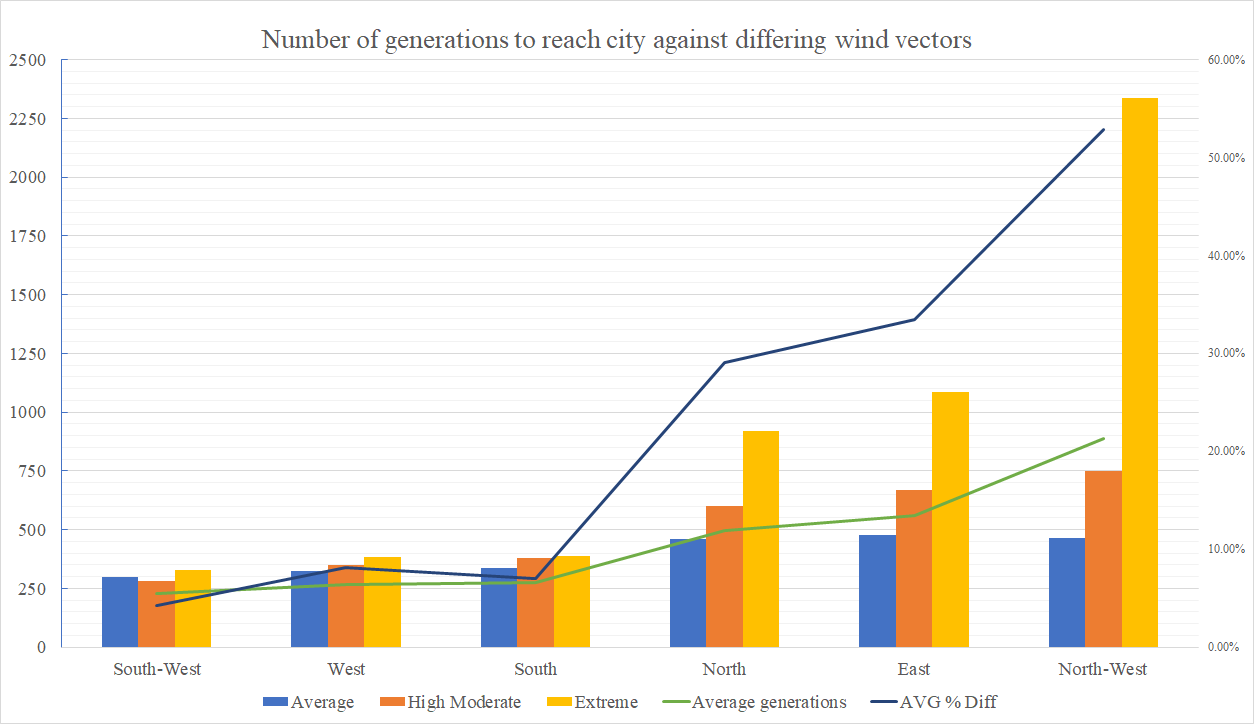
\includegraphics[width=\linewidth]{imgs/graphs/wind.png}
      \caption{Graph showing the number of generations taken to reach the city against differing wind speeds.}
      \label{}
    \end{figure}

    % There are two notable values in the wind data that could be seen as outliers, and such deserve discussion.
  



    \begin{figure}[H]
      \centering
      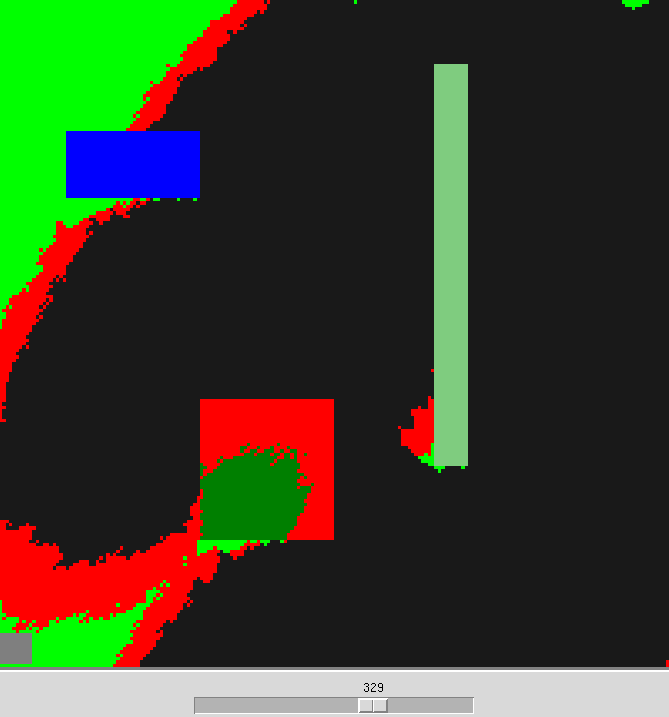
\includegraphics[width=0.75\linewidth]{imgs/wind/x-15y15_gen329}
      \caption{In extreme South Westerly winds, the fire is affected by the placement of the dense forest, canyon, and water, such that the spread towards the town is slower than that of a fire with lower wind speeds.}
      \label{}
    \end{figure}


    \begin{figure}[h]
      \centering
      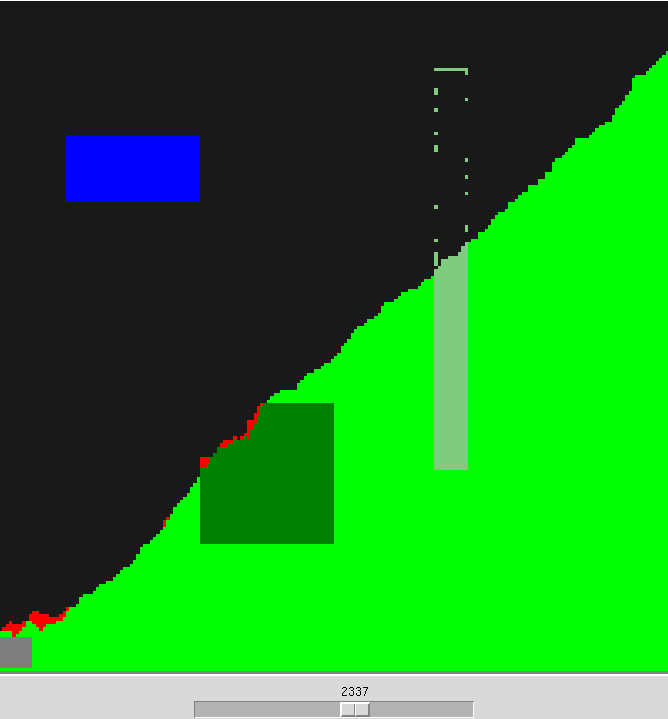
\includegraphics[width=0.75\linewidth]{imgs/wind/x-15y-15_gen2337}
      \caption{In extreme North Westerly winds, the majority of the fire spread misses the town. It is only after roughly 2100 generations does the fire eventually spread in the south direction enough to reach the town.}
      \label{}
    \end{figure}
    % \subsubsection{No Wind}

    % \subsubsection{East to West}
    % \subsubsection{North to South}
    % \subsubsection{North East}
    % \subsubsection{South West}

  % \subsection{Resolution     -  50 x  50}
  % \subsection{Resolution     - 200 x 200}
  % \subsection{Resolution     - 400 x 400}



  % \begin{table}[H]
  %   \begin{tabular}{|l|l|l|l|l|l|l|}
  %   \hline
  %   Top left & Bottom right & gen reached & dump gen & gen diff & gens to reach & +/- \\ \hline
  %   130, 140 & 140, 150     & 172                          & 182      & 10       & 298           & -8  \\ \hline
  %   190 ,200 & 200, 10      & 0                            & 14       & 14       & 302           & -4  \\ \hline
  %   80,75    & 90,85        & 150                          & 0        & -150     & 303           & -3  \\ \hline
  %   130,10   & 140,20       & 77                           & 0        & -77      & 303           & -3  \\ \hline
  %   130, 140 & 140, 150     & 172                          & 172      & 0        & 304           & -2  \\ \hline
  %   \textbf{-}        & \textbf{-}            &\textbf{ }-                            & \textbf{-}        & \textbf{-}        & \textbf{306}           & \textbf{0}   \\ \hline
  %   10,190   & 20,200       & 295                          & 305      & 10       & 306           & 0   \\ \hline
  %   80,100   & 90,110       & 157                          & 167      & 10       & 306           & 0   \\ \hline
  %   130,10   & 140,20       & 77                           & 87       & 10       & 306           & 0   \\ \hline
  %   10, 182  & 20, 192      & 290                          & 300      & 10       & 307           & 1   \\ \hline
  %   10, 182  & 20, 192      & 290                          & 0        & -290     & 308           & 2   \\ \hline
  %   80,100   & 90,110       & 157                          & 0        & -157     & 309           & 3   \\ \hline
  %   80,100   & 90,110       & 157                          & 157      & 0        & 309           & 3   \\ \hline
  %   80, 75   & 90, 85       & 150                          & 160      & 10       & 309           & 3   \\ \hline
  %   10,190   & 20,200       & 295                          & 300      & 5        & 310           & 4   \\ \hline
  %   80, 75   & 90, 85       & 150                          & 150      & 0        & 310           & 4   \\ \hline
  %   130,10   & 140,20       & 77                           & 77       & 0        & 311           & 5   \\ \hline
  %   190 ,200 & 200, 10      & 0                            & 15       & 15       & 312           & 6   \\ \hline
  %   190 ,200 & 200, 10      & 0                            & 20       & 20       & 312           & 6   \\ \hline
  %   130, 140 & 140, 150     & 172                          & 0        & -172     & 312           & 6   \\ \hline
  %   10, 182  & 20, 192      & 290                          & 295      & 5        & 313           & 7   \\ \hline
  %   10,190   & 20,200       & 295                          & 0        & -295     & 314           & 8   \\ \hline
  %   190 ,200 & 200, 10      & 0                            & 0        & 0        & -             & -   \\ \hline
  %   190 ,200 & 200, 10      & 0                            & 13       & 13       & -             & -   \\ \hline
  %   \end{tabular}
  %   \end{table}
  \subsection{Best water locations}
  Due to the small size of the water available, ensuring the timely deposit of the water is essential to its effectiveness.

  By experimenting with different water locations across the grid, and comparing the amount of time it takes for the fire to reach the city, it is possible to devise an optimal location. Setting the wind values to 0 helps remove any wind effects from our initial calculations.

  Due to the nature of this solution's implementation, the time step at which water can be dropped can be adjusted. Because this system simulates an `airdrop' of water, it was important to try and simulate the effects of the water being dropped at various different points in time, and at different points on the fire front.

  \subsubsection{Choosing locations}
  It is important in our assessment of optimal water location to choose the best areas to sample, not least due to the small size of the water available ($10km^2$). \cite{christopher_2019} suggests the optimal placing of water in a forest fire is near the source, and on the `attacking front' of the fire.

  To this end, the following water placements were devised:

  \begin{itemize}
    \item[(190, 200).]  The top right. What would happen if the fire could be stopped early into its journey?
    \item[ (10, 190).] Bottom right hand side of the town. A similar tactic as above. These are the nearest two sides to the wildfire front.
    \item[(130,140).] The southern end of the canyon - similar tactic.
    \item[ (80, 100).] Between the lake and the dense forest - Does decreasing this area make a difference?
    \item[ (10,182).] The top of the town. If for whatever reason it wasn't feasible for the crews to reach the start of the fire, would an effective preventative measure be blocking the surrounding area near the town?
    \item[ (80, 75).] The same tactic but closer to the lake    
    \item[(130,10).] The northern end of the canyon - This is to try and make a blockade which extends the journey of the fire.
  \end{itemize}

  \subsubsection{Results}


    \textit{Default number of generations: 306} \\
    $c$ is the generation at which the fire reaches the water's eventual location. \\
    $gens_{x}$ is the number of generations it takes for the fire to reach the town when the water is placed at generation $x$.

  % Change to one column?
      \begin{table}[H]
        \begin{tabular}{|l|l|l|l|l|l|l|l|}
        \hline
        Water coordinates    &  $c$ & $gens_0$ & $gens_{c}$ & $gens_{c+10}$ & $\Delta gens_0$ & $\Delta gens_c$ & $\Delta gens_{c+10}$ \\ \hline
        (190, 200), (200,10) & 0   & $\infty$     & $\infty$       & $\infty$         & $\infty$        & $\infty$        & $\infty$           \\ \hline
        (10, 190), (20,200)  & 295 & 314   & 310     & 306       & 8        & 4        & 0           \\ \hline
        (130,140), (140, 15) & 172 & 312   & 304     & 298       & 6        & -2       & -8          \\ \hline
        (80,100),(90,11)     & 157 & 309   & 309     & 306       & 3        & 3        & 0           \\ \hline
        (10,182), (20, 192)  & 290 & 308   & 313     & 307       & 2        & 7        & 1           \\ \hline
        (80, 75), (90,85)    & 150 & 303   & 310     & 309       & -3       & 4        & 3           \\ \hline
        (130,10), (140, 20)  & 77  & 303   & 311     & 306       & -3       & 5        & 0           \\ \hline
        \end{tabular}
        \end{table}

        \begin{figure}[h]
          \centering
            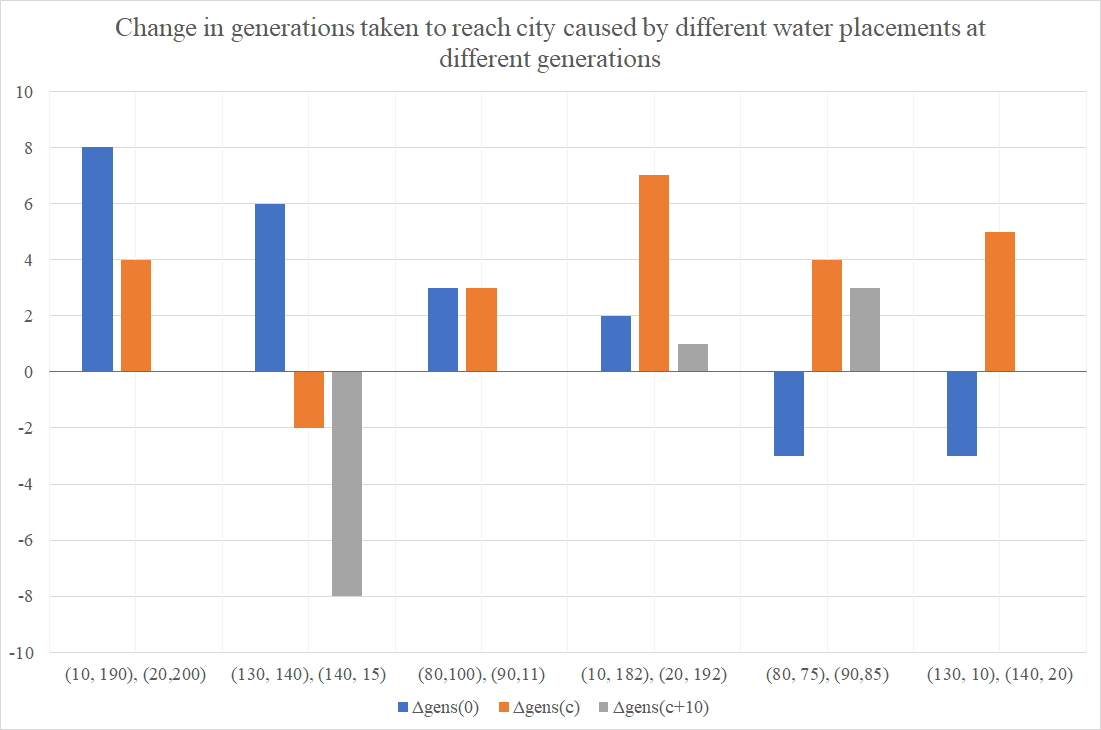
\includegraphics[width=\linewidth]{imgs/graphs/water_gens.png}
          \caption{Graph showing the change in generations taken to reach city, caused by the differing water placements at different generations.}
          \label{}
        \end{figure}
      % Because SW wind produced the a fire front which met the town the quickest, and dropping water at $\Delta gens_c$ produced the greatest increase to generations on average, testing different water locations within this domain was also performed.



      



\subsection{Dense forest locations}
There is the opportunity to add additional dense forest to the terrain, vai extension of the existing block. Choosing the best extension of this forest is a trial and error process, for which the following extensions were consulted:
 \begin{itemize}
   \item Double the width, the additional on the west side
   \item Double the width, the additional on the east side
   \item Double the width, the additional split equally on both sides
   \item Double the height, the additional on the north side
   \item Double the height, the additional on the south side
   \item Double the height, the additional split equally on both sides

 \end{itemize}

 \begin{table}[H]
  \centering
  \begin{tabular}{|l|l|}
  \hline
  Direction & generations \\ \hline
  default & 306 \\ \hline
  \textbf{to E}    & \textbf{328} \\ \hline
  to W    & 309 \\ \hline
  W + E   & 313 \\ \hline
  to N    & 326 \\ \hline
  to S    & 304 \\ \hline
  N + S    & 326 \\ \hline
  
  
  
  
  \end{tabular}
  \end{table}

  Because SW wind produced the a fire front which met the town the quickest, analysing dense forest location within this domain was also performed.

  \begin{table}[H]
    \centering
    \begin{tabular}{|l|l|}
    \hline
    Direction & generations \\ \hline
    default & 296 \\ \hline
    \textbf{to E}    & \textbf{354} \\ \hline
    to W    & 327 \\ \hline
    W + E   & 301 \\ \hline
    to N    & 334 \\ \hline
    to S    & 282 \\ \hline
    N + S    & 323 \\ \hline
    
    
    
    
    
    \end{tabular}
    \end{table}

\newpage
\section{Discussion of model and conclusions} 
\section{Conclusion}

\newpage
\renewcommand{\bibname}{References}
\bibliographystyle{apacite}
\bibliography{Bibliography.bib}


\end{document} 